\documentclass[12pt,a4j]{jarticle}
\usepackage[dvipdfm]{graphicx}
\usepackage{musixtex}
\begin{document}
\title{jazz guitar初心者向け資料}
\maketitle

\section{メジャースケールとダイアトニックコード}
Cメジャースケールを弾いて、と言われてパッと弾くことができるでしょうか。おそらく殆どの人が楽器に初めて触ったときに弾けるようになったであろう「ドレミファソラシド」です。
Fメジャースケールを弾いてと言われれば「F-G-A-B$\flat$-C-D-E-F」となり、E$\flat$メジャースケールを弾いてと言われれば「E$\flat$-F-G-A$\flat$-B$\flat$-C-D-E$\flat$」となります。


まずはCメジャースケールを各ポジションで弾けるようになりましょう。ギターの5弦の3フレットのCから1限の8フレットのCを1、2パターン程度、6弦8フレットから1限の8フレットのC、または2弦13フレットのC、5弦15フレットのCから2弦13フレットのCに向かう5パターン程度を淀みなく弾けるように練習しましょう。
なれてきたらCから4度先のメジャースケールを練習していきましょう。F、B$\flat$、E$\flat$、A$\flat$、D$\flat$、G$\flat$、B、E、A、D、Gとちょうど12音すべてのメジャースケールが練習できるはずです。

\vskip\baselineskip
これらのメジャースケールを3度ずつ(1音ずつ飛ばした)4つの音を堆積していったものがコードになります。これをメジャーダイアトニックコードと呼びます。
ここにCメジャーダイアトニックコードを一通り示します。

\vskip\baselineskip
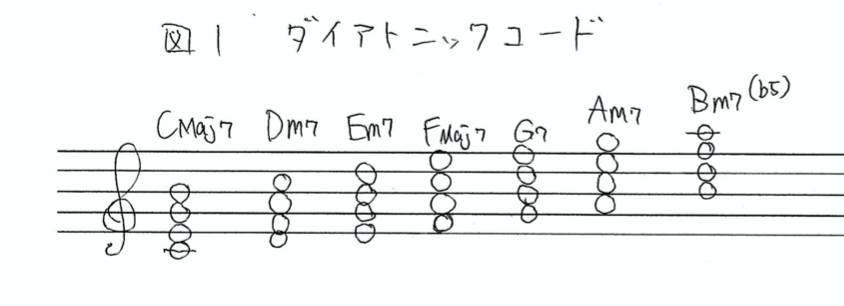
\includegraphics{diatonic.png}

\section{基本コード}
ここからはコードの押さえ方を解説します。ジャズのコードと言われればテンションコード等複雑なものを思い浮かべますがここではシンプルなコードを覚えていきましょう。
そのためにはまず5弦ルート、6弦ルートという考え方を知らなければいけません。例えばDm7を弾きたいとします。名前の通り、間違えなくDの音が入ってることがわかりますね。これがルート音と呼ばれる音です。
まずは5弦、6弦からDの音を探してみましょう。


ルート音が探せたならば他の構成音を探してみましょう。さっきのダイアトニックコードの表をみると、Dm7はDの他にF、A、Cの音があることがわかります。これらの音をルート音で選んだ弦以外から選んで押さえればDm7の完成です。

といってもそんなに簡単に探すことはできませんね。ここで度数という考え方を取り入れたいと思います。
先程のメジャースケールの練習法でも4度先という表現を使いました。これは基準の音から4度離れた音という意味になります。完全4度(Perfect 4th)と呼びます。
度数について細かい定義を知りたい方は楽典等を参考にしてください。今回はコードの説明のために簡単に度数の概念について説明します。

\vskip\baselineskip
Cの音を1度とするとDは2度、Eは3度、Fは4度、Gは5度、Aは6度、Bは7度となります。順番に弾いてみるとCメジャースケールになることがわかると思います。メジャースケールの順番が1から7までの度数と覚えましょう。

メジャースケールの度数を覚えれたら、もう少し細かい区分の名前があるのでそれを覚えましょう。メジャースケールの2、3、6、7度の音を長音程と呼ぶので、それぞれ長○度、もしくはメジャー○度と呼びましょう。残った1、4、5度の音を完全音程と呼ぶので完全○度と覚えましょう。
そして長音程を半音下げた音(フレット1つ分左)を短音程と呼ぶので短○度と覚えましょう。長2度の半音下は短2度というようにそれぞれ名前が付きます。これらすべて一つずつ数えると1オクターブを均等に割った12音階が見えてくるはずです。
また、音の順番を変えてみる、例えば1度から完全音の関係の順番を1オクターブ上の1度と入れ替えるとその完全音からオクターブ上の1度は完全音の関係になるというのと、1度と長音程の関係の順番をその長音程と1オクターブ上の1度に入れ替えたら短音程の関係になるということを覚えておくと便利です。
この順番を入れ替えることを転回と呼びます。完全4度の音程を転回すれば完全5度、短3度の関係を展開すれば長6度の音程になります。
\vskip\baselineskip
余談ですが、現代では当たり前に12音階を使って音楽が作られていますが、世界の民族音楽の中には12音階ではないものももちろんあります。日本の昔の音楽は三部損益法というメソッドから割り出した12律からできているものがありますが、西洋音楽のそれとはすこし違っていたりします。
また平均律と純正律も音楽の面白いテーマだと思います。それぞれ興味があれば調べてみてください。

\vskip\baselineskip

ここでコードの話に戻ります。ダイアトニックコードをもう一度参照してみましょう。コードの種類は○Maj7、○m7、○7、○m7♭5があると思います。まずこれらのコードの6弦ルートからのコードを示します。

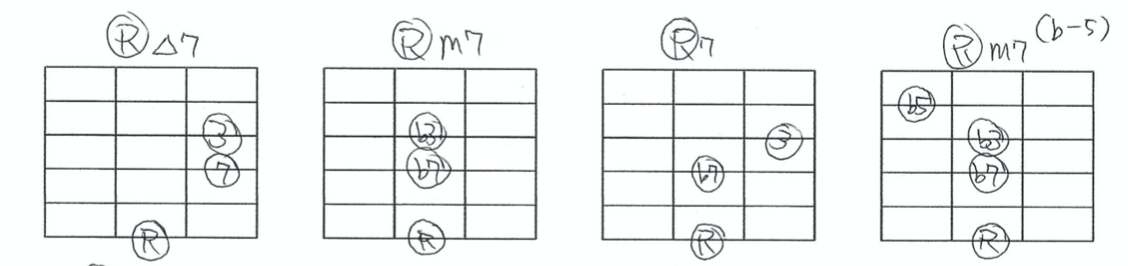
\includegraphics[width=150mm]{6root.png}

それぞれ意味を説明します。○が指で押さえる箇所でRがルート音、数字が度数を表しており、♭がついていれば短○度、なければ長○度となります。ここでメジャーダイアトニックコードの図と見比べてみると○m7♭5以外は完全5度の音が入っていないことがわかると思います。まずはこの完全5度の音を抜いた3voiceと呼ばれるシンプルなコードをマスターしましょう。

\vskip\baselineskip
同様に5弦ルートのコードも示します。

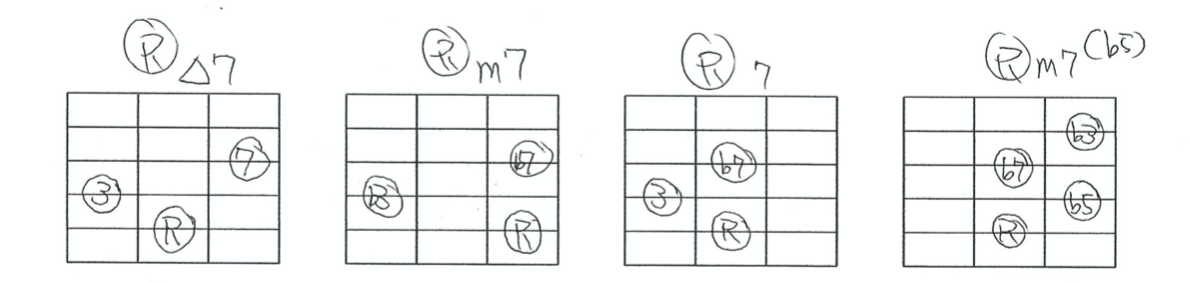
\includegraphics[width=150mm]{5root.png}

これだけ覚えればセッションに参加することが可能になります。そしてさらに別の響きのコードを鳴らしてみたいと思ったとき、度数について覚えたことが役に立ちます。
指示されたコード内の音をさっきの基本コードから足してみたり、転回して組み替えてみたりしましょう。様々なハーモニーが楽しめると思います。なかには良い響きではない組み合わせもあるでしょう。
自分が良いと思ったコードをセッションの場面でどんどん試していってください。

ときには♭9のような今までの説明ではなかったコードを指示されたりしますが、これまでの考え方を応用すれば対応できるはずです。

また教則本などに載ってるコードを覚えるときもルート音からの音程を意識して覚えるようにしましょう。
\end{document}